\chapter{Analysis}
\label{chap:num_3}

The following chapter will start by providing a detailed set of functional and non-functional requirements from \lpa{} in regards to \lpas{}. Afterward, an analysis of the currently available development tools within the \solid{} ecosystem will be demonstrated. Additionally, as a continuation of comparison in \autoref{sssec:comparison_of_technologies}, a reasoning for choosing \solid{} as a core technology for implementing \lpa{} requirements will be explained.  The majority of the functionality of \lpa{} and \lpas{} were implemented by the author while working in parallel as a part of \lpa{} and as an individual contribution to the thesis. Therefore, to simplify the understanding of work on both projects and the difference between both contributions, the whole chapter is structured under the assumption that \lpa{} is a stakeholder with a working solution and \lpas{} is a technology yet to be implemented and integrated into \lpa{}. The consecutive chapter on architecture in \autoref{chap:num_4} and the implementation in \autoref{chap:num_5}, will guide the reader through established software development cycles where the result will be provided as a summary of implementation details in regards to requirements defined in this chapter.

Aside from definitions of specific requirements, it is important to note that there are three main \textit{actors} involved in statements of requirements. An actor is an individual entity interacting with the software components in requirements. Specific types are defined as follows:
\begin{itemize}
    \item \textit{Data journalists}, this category of actors are one of main target users of \lpa{} platform. They are defined as people familiar with, at least, basics of Semantic Web. They can provide Linked  Data sources to \lpa{} for further visualization and publishing of apps. They are also assumed to have an actual account in the \lpa{} platform.
    \item \textit{Lay users}, this is a second target category of users of \lpa{} platform. They do not have any prior experience with Semantic Web and in most cases, browse the published visualizers created by Data journalists. They are not obliged to have an actual account in the \lpa{} platform.
    \item \textit{\acrfull{LPA} Developers}, a developers implementing on \lpa{} platform codebase and main users of \lpas{} features, APIs and functionality to be developed. The majority of details in \autoref{chap:num_5} are focused on developing a developer-friendly software for this category of users.
\end{itemize}

\section{Functional requirements}
\label{ssec:functional_requirements}

In general, every functional requirement is defined as a description of services or features that software must offer. In this case \lpa{} defines a set of features expected to be handled properly by the \lpas{} project. The requirements are provided as a set of UML use-case \footnote{\url{https://www.uml-diagrams.org/use-case-diagrams.html}} diagrams as well as formal textual descriptions. 

\subsection{User authentication}

The user of the platform should be able to register an account in the application, log in, and log out. The requirement might seem unfitting to the purposes of \lpas{}. However, if \solid{} is considered to be used, it provides the fully functional authentication mechanisms based on WebID that can be used for generic platform authorization.

\begin{figure}[h]
\centering
\fcolorbox{black}{white}{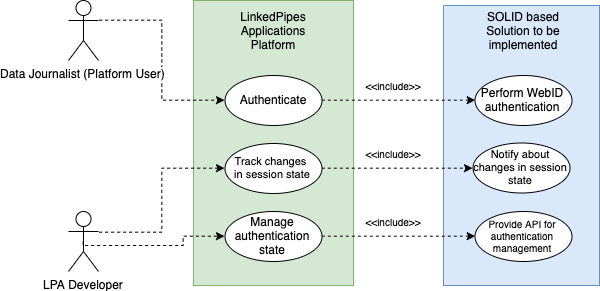
\includegraphics[width=0.7\linewidth]{lpa_authenticating_use_case.png}}
\caption{A UML use-case diagram describing user authentication requirement.}
\label{fig:lpa_authenticating_use_case}
\end{figure}

The UML diagram on \autoref{fig:lpa_authenticating_use_case} is described as follows:
\begin{itemize}
    \item \textit{Authenticate}, a platform must provide a way for Data Journalists (Platform Users) to authenticate via \lpa{} platform. This assumes that \lpa{} platform has an ability to communicate with the storage solution either integrated into \lpa{} codebase or presented as entirely separate service and \textit{perform WebID authentication}.
    \item \textit{Track changes in session state}, a platform must provide an API or a developer library for tracking any changes in the state of the authenticated platform user session. This assumes that the storage solution can inform the \lpa{} platform about such changes.
    \item \textit{Manage authentication state}, the platform must provide an API or a developer library for managing the authentication state of the users. This assumes that the core functionality is provided by the storage solution that exposes an API or a developer library toolset for developers to perform such interactions.
\end{itemize}

\subsection{Create, Store and Publish Application}

Creation, storing, and publishing of the application are the core features provided by the \lpa{} itself. However, the storage aspects are involved a lot when it comes to storing the created app. Consequently, publishing also consists of interacting with storage since an end-user expects the storage solution to have an identifier for his stored application.

\subsubsection{Creating and storing application}

User should be able to create an application within the \lpa{} platform and store it in his personal space in an authenticated storage. The storage solution can either implement a solution that stores entire application including the visualizer or generates a metadata configuration file that allows to re-create the entire application within \lpa{} platform from scratch.

\subsubsection{Publishing an application}

Another important requirement is an ability to publish the application and make it publically available for sharing the visualization to anyone via the permanent link. Furthermore, when a third party accesses this \textit{permalink}, the browser should open the \lpa{} website with the respective application opened, as configured by the publisher. The tool will also need to provide the ability to embed the published view into a data journalist's web page, for example, using an HTML \texttt{iframe} \footnote{\url{https://html.com/tags/iframe}}. 

\subsubsection{A diagram overview}

The \autoref{chap:num_5} describes the specific of creation, storing and publishing application requirements from perspectives of different actors involved. 

\begin{figure}[h]
\centering
\fcolorbox{black}{white}{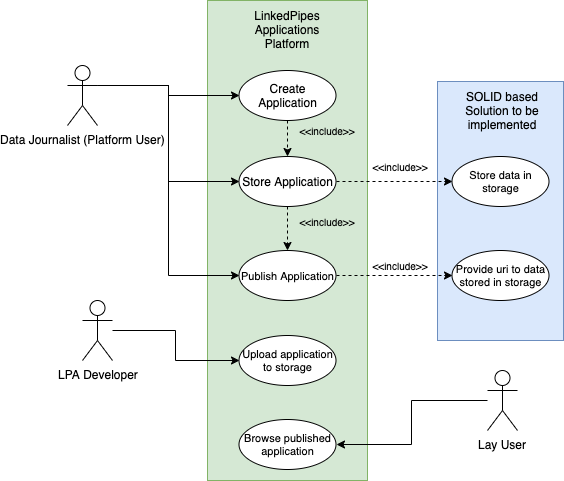
\includegraphics[width=0.6\linewidth]{lpa_creating_apps_use_case.png}}
\caption{A UML use-case diagram describing creation, storing and publishing application requirements.}
\label{fig:lpa_creating_apps_use_case}
\end{figure}

The diagram is described as follows:
\begin{itemize}
    \item \textit{Create application}, the platform provides an ability for Data Journalists to create an application. The process of creation of an application within \lpa{} also assumes that it is consequently \textit{Stored} and \textit{Published} via a set of interactions with storage. The publishing process is extended from storing an application because to publish an application, a configuration needs to be saved, and a URI for a stored resource in a \solid{} POD is extracted.
    \item \textit{Upload application to storage}, a platform provides an API or a library for LPA Developers to perform uploading of an application into the storage solution.
    \item \textit{Browse published application}, a platform provides a way for any Lay User to browse the published application created by Data Journalists. This is included as a part of the requirement since publishing is directly interacting with storage, and implementation of the requirement applies to both \lpas{} and \lpa{} platform.
\end{itemize}


\subsection{Managing storage and sharing published applications}

The last set of requirements is related to storage management and the sharing of published applications. The storage management requires a functionality that allows platform users to \textit{move}, \textit{copy} and \textit{create} data in their authenticated spaces in storage. The sharing requirement describes the functionality to allow users to share the applications they have published and control the access control settings to them. Since published applications require to be publically accessible to anyone, the platform needs to have a functionality to persist the configurations of the applications in a secure way. Moreover, the configurations for most of the published applications are represented as Linked Data. Therefore the persistent storage tooling needs to be optimized for files in RDF format.
 
\begin{figure}[h]
\centering
\fcolorbox{black}{white}{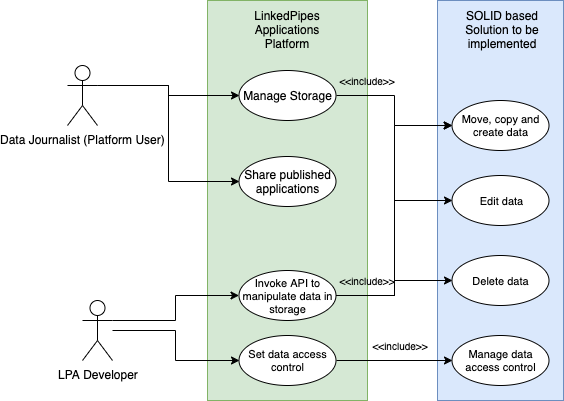
\includegraphics[width=0.6\linewidth]{lpa_managing_storage.png}}
\caption{A UML use-case diagram describing requirements on storage management and sharing of published application.}
\label{fig:lpa_managing_storage}
\end{figure}

As demonstrated on \autoref{fig:lpa_managing_storage}, the main elements are described as follows:
\begin{itemize}
    \item \textit{Manage storage}, the functionality of the platform to allow Data Journalists (Platform Users) to interact and manipulate data in their storage. In the case of \lpa{}, it is limited to visualizer application-related data only. 
    \item \textit{Share published applications}, an ability for Data Journalists to share the application with other users of the \lpa{} platform and set access control to the published applications.
    \item \textit{Invoke API to manipulate data in storage} assumes that \lpa{} provides tooling for their developers to interact with storage solution and invoke its APIs or libraries for manipulating data.
    \item \textit{Set data access control}, assumes that \lpa{} provides tooling for their developers to interact with storage solution and invoke its APIs or libraries for editing access control privileges to data.
\end{itemize}

\section{Non-functional requirements}
\label{ssec:non_functional_requirements}

In general, every non-functional requirement is described as the quality attributes of a software system, which contrasts with functional requirements that are specific to the exact behavior of the system. Within the scope of \lpa{} platform, the stated non-functional are rather an informal set of terms mainly related to \textit{reusability}, \textit{testability} quality attributes. 

\subsection{Compatibility with latest tools}

This general non-functional requirement states that an implemented software solution should be compatible with the latest tools of its technological ecosystem. For instance, if the designed software is a library using third-party packages, it needs to be generic enough to be compatible or have mechanisms to be resilient to any significant changes in third-party packages that it relies on.

\subsection{Clean APIs and libraries}

The solution needs to be implemented with code readability and reusability in mind. The primary users of the solution are developers of \lpa{} platform. Therefore it is essential to have an implementation based on a design that minds the established best practices and patterns of software engineering. 

\subsection{Continuous Integration and Delivery}

The implemented solution needs to maintain an optimized and fully automated Continuous Integration and Delivery pipelines. This ensures better possibilities in gaining contributors and planning future work and improvements on the solution as well as an infrastructure to debug and fix errors more effectively.

\subsection{Easy integration with \lpa{}}

The final solution needs to be able to integrate with the \lpa{} easily. Another important aspect is the solution to be integrated should not be entirely tied to the specified \lpa{} platform and should have the potential to be reused in other Linked Data based applications.

\subsection{Decentralized storage}

The Data Journalists, one of the primary target users of \lpa{} platform, should be able to choose any storage that is compliant with the technology stack of the solution. In other words, the platform should be able to support storing data in any personal space of such storage instances that are created, hosted, or owned by users directly or by the third-party providers.

\section{\solid{} development toolset}

Now, as the main requirements of the \lpa{} platform are defined, let us dive into the analysis of the \solid{} technology and tooling that it provides to understand better how it can be used to cover all stated requirements.

At the core \solid{} is a set of open specifications. At the current state of the project implementation, the community is most concerned about the persistence and representation of resources. However, such aspects as identity, authentication, and authorization are also vital parts of \solid{}.

A set of these standards are undergoing active implementation stage. Main contributors consisting of the core \solid{} development team, as well as the open-source community, develop the standards into various servers and tools. For instance, a \texttt{node-solid-server} library that implements a Solid server in Node and \texttt{rdflib.js} that allows you to manipulate RDF programmatically.

In addition to this, there is work done on supporting tools, such as Solid React SDK, that is created to allow developers to more easily get into developing apps with Solid. As part of this is the style guide that can be reused by others, not wanting to use the React parts.

\subsection{The \solid{} servers}

\solid{} itself represents a tech stack of complementary standards and data format vocabularies that are currently only available in centralized social media services. It also represents a Specification Document, serving as the main guideline for developers building their own apps and services. However, aside from that \solid{} also refers to a set of servers that implement its specification. 

\subsubsection{gold}

\texttt{gold} is a reference Linked Data Platform server for the \solid{} platform. The implementation is written in Go, based on initial work done by William Waites \cite{solid_gold_server}.

\subsubsection{node-solid-server}

Following solution is an implementation of a server based on \solid{} specifications in Node.js \cite{node_solid_server}.
One of the main advantages is that it could be launched as a \solid{} server on top of the local file-system. Interaction with server can be performed as follows:
\begin{itemize}
	\item Command line tool.
    \item Via \texttt{node-solid-server} library.
\end{itemize}

The provided server implementation was used as a main \solid{} server for the project due to compliance with main requirements for choosing the server. Those can be described as follows:
\begin{itemize}
	\item \textbf{Easy integration with current \lpa{} project}, specifically the frontend web project. This allows usage of provided `node-solid-server.js` library.
    \item \textbf{Active maintenance by open-source community}. Aside from that, this server implementation is considered to be a default option suggested by creators of \solid{}.
    \item \textbf{Support of \textit{WebID-TLS} and \textit{WebID-OIDC}}. This implies majority of WebID communications protocols,
    crucial to the user authentication and security aspects of the storage within \lpa{}. The WebID-TLS stands for a WebID authentication method over \acrfull{TLS}, providing an efficient and user friendly authentication on the Web \cite{webid_tls}. The WebID-OIDC is an authentication delegation protocol suitable for WebID-based decentralized systems such as \solid{} \cite{webid_oidc}.
\end{itemize}

\subsection{The \solid{} React development stack}

The main frontend library used in LinkedPipes Applications is React. In order to incorporate easier integration of aspects of \solid{} into the project, an analysis of React related \solid{} frameworks and libraries was performed. Even though, \solid{} community is yet to grow become stable and mature, it already provides a convenient set of libraries for React that were used as a main tools during implementation of the thesis project. 

\subsubsection{solid/react}

The main purpose of this library is to provide the following functionality:

\begin{itemize}
	\item Provide React developers with components to develop \solid{} apps.
    \item Enable React developers to build their own components for \solid{}.
\end{itemize}

\subsubsection{@inrupt/solid-react-components}

This libray is an official SDK provided by Inrupt for developing React Web applications for \solid{}. The package include various dependencies allowing:

\begin{itemize}
	\item Provide React developers with a set of easily customizable components interacting with \solid{} specifications.
    \item Provide a standardized visual design conventions based on Atomic Style.
    \item A set of cli commands for generating a template \solid{} projects.
\end{itemize}

\subsubsection{solid-auth-client}

The main purpose of this low level library is to provide ability to easily perform Authentication operations while interacting with \solid{} pods and servers.

At its core it is a browser library that allows your apps to securely log in to \solid{} data pods and read and write data from them.

\subsubsection{solid-file-client}

This library provides a simple interface for logging in and out of a Solid data store, maintaining a persistent session, and for managing files and folders. It may be used either directly in the browser or with node/require. The library is based on solid-auth-client and solid-cli, providing an error-handling interface and some convenience shortcuts on top of their methods and providing a common interface to the two modules.

\subsubsection{rdflib}

JavaScript RDF library for browsers and Node.js. One of the main contributors is Sir Tim Berners-Lee himself. The library is going to be used and described in detail in \autoref{chap:num_5}.

\subsubsection{@solid/query-ldflex}

The following library adds support of the LDflex language to \solid{} by:

\begin{itemize}
	\item Providing a JSON-LD context for \solid{}.
    \item Binding a query engine (Comunica).
    \item Exposing useful data paths.
    \item LDflex expressions occur for example on Solid React components, where they make it easy for developers to specify what data they want to show. They can also be used as an expression language in any other Solid project or framework.
\end{itemize}

\section{Why \solid{}?}
\label{sssec:why_solid}

Even though it is presented as a flawless dominating technology in \autoref{table:solid_comparisons_table}, it is, in fact, far from being perfect. Some of the disadvantages include:
\begin{itemize}
    \item \textit{Still under active research and development}, the project itself started back in 2016. Still, the real active traction and improvements had happened only within the past two years after community grew bigger, and the project gained popularity in the open-source community. It also means that there are still major changes in specifications introduces in every new iteration.
    \item \textit{Lack of actively maintained community libraries}, even though \solid{} organization on GitHub \footnote{\url{https://github.com}} actively updates and maintains its libraries for interacting with \solid{}. There is a large number of libraries developed by the community with tools that, in some cases, are more useful and popular. However, due to the \solid{} project still being actively developed, a lot of libraries outside of the scope of the organization become obsolete and outdated quickly.
    \item \textit{Still a lot of room for improving infrastructure for developers}. The project does not provide intuitive and user-friendly documentation. An average developer is required to have basic knowledge in Semantic Web, Linked Data, and working with RDF and SPARQL. However, the improvements were made in 2019, and eventually, the onboarding process into the technology will become easier for any developer.
\end{itemize}

Despite the disadvantaged mentioned above, the main reason for choosing \solid{} as a core for providing storage capabilities to \lpa{} was the fact that it is a very flexible and low-level technology.  Firstly,  as mentioned earlier, \solid{} represents multiple things at once. It is both a toolset with libraries for developers, a set of specifications, and an ambitious idea to a better World Wide Web where people own their data, and all information is linked together, preserving the semantic meaning. Of course, many attempts on decentralization were made before, but \solid{} differs from the others in the way that it does not target individuals in specific fields or domains of the Internet, it attempts to change the Internet itself, making it a better online space for everyone. And lastly, it demonstrated itself as a perfect fit for any application that requires any social aspects and involves dealing with any form of Linked Data, where \lpa{} platform and its requirements are compliant to all of the statements mentioned earlier.